\documentclass[12pt]{beamer}
\usepackage{../Estilos/BeamerMAF}
\usetheme{Dresden}
\usecolortheme{seahorse}
%\useoutertheme{default}
\setbeamercovered{invisible}
% or whatever (possibly just delete it)
\setbeamertemplate{section in toc}[sections numbered]
\setbeamertemplate{subsection in toc}[subsections numbered]
\setbeamertemplate{subsection in toc}{\leavevmode\leftskip=3.2em\rlap{\hskip-2em\inserttocsectionnumber.\inserttocsubsectionnumber}\inserttocsubsection\par}
\setbeamercolor{section in toc}{fg=blue}
\setbeamercolor{subsection in toc}{fg=blue}
\setbeamercolor{frametitle}{fg=blue}
\setbeamertemplate{caption}[numbered]

\setbeamertemplate{footline}
\beamertemplatenavigationsymbolsempty
\setbeamertemplate{headline}{}

\makeatletter
\setbeamercolor{section in foot}{bg=gray!30, fg=black!90!orange}
\setbeamercolor{subsection in foot}{bg=blue!30!yellow, fg=red}
\setbeamertemplate{footline}
{
  \leavevmode%
  \hbox{%
  \begin{beamercolorbox}[wd=.333333\paperwidth,ht=2.25ex,dp=1ex,center]{section in foot}%
    \usebeamerfont{section in foot} \insertsection
  \end{beamercolorbox}}%
  \begin{beamercolorbox}[wd=.333333\paperwidth,ht=2.25ex,dp=1ex,center]{subsection in foot}%
    \usebeamerfont{subsection in foot}  \insertsubsection
  \end{beamercolorbox}%
  \begin{beamercolorbox}[wd=.333333\paperwidth,ht=2.25ex,dp=1ex,right]{date in head/foot}%
    \usebeamerfont{date in head/foot} \insertshortdate{} \hspace*{2em}
    \insertframenumber{} / \inserttotalframenumber \hspace*{2ex} 
  \end{beamercolorbox}}%
  \vskip0pt%
\makeatother 

\makeatletter
\patchcmd{\beamer@sectionintoc}{\vskip1.5em}{\vskip0.8em}{}{}
\makeatother


\setbeamercolor{section in foot}{bg=darkspringgreen, fg=white}
\setbeamercolor{subsection in foot}{bg=persianblue, fg=white}
\setbeamercolor{date in foot}{bg=goldenrod, fg=white}

\makeatletter
\setbeamertemplate{footline}
{
  \leavevmode%
  \hbox{%
  \begin{beamercolorbox}[wd=.333333\paperwidth,ht=2.25ex,dp=1ex,center]{section in foot}%
    \usebeamerfont{section in foot} \insertsection
  \end{beamercolorbox}%
  \begin{beamercolorbox}[wd=.333333\paperwidth,ht=2.25ex,dp=1ex,center]{subsection in foot}%
    \usebeamerfont{subsection in foot}  \insertsubsection
  \end{beamercolorbox}%
  \begin{beamercolorbox}[wd=.333333\paperwidth,ht=2.25ex,dp=1ex,right]{date in head/foot}%
    \usebeamerfont{date in head/foot} \insertshortdate{} \hspace*{2em}
    \insertframenumber{} / \inserttotalframenumber \hspace*{2ex} 
  \end{beamercolorbox}}%
  \vskip0pt%
}
\makeatother
\usefonttheme{serif}
\resetcounteronoverlays{saveenumi}

\date{24 de marzo de 2022}

\title{\large{Teoría Sturm-Liouville}}
\subtitle{Tema 3 - Bases completas y ortogonales}
\author{M. en C. Gustavo Contreras Mayén}


\begin{document}
\maketitle
\fontsize{14}{14}\selectfont
\spanishdecimal{.}

\section*{Contenido}
\frame[allowframebreaks]{\tableofcontents[currentsection, hideallsubsections]}


%Ref. Herman (2015)  - Sturm-Liouville
\section{Problemas de tipo Sturm-Liouville.}
\frame{\tableofcontents[currentsection, hideothersubsections]}
\subsection{Introducción}

\begin{frame}
\frametitle{Soluciones a las EDO}
Hemos visto que las funciones trigonométricas y que algunas las funciones especiales son las soluciones de ecuaciones diferenciales.
\\
\bigskip
\pause
Estas soluciones dan conjuntos ortogonales de funciones que se pueden utilizar para representar funciones en expansiones de series de Fourier generalizadas.
\end{frame}
\begin{frame}
\frametitle{Procedimientos más generales}
Al mismo tiempo, sería interesante generalizar las técnicas que usamos por primera vez para resolver la ecuación de calor con el fin de resolver problemas más generales de valores iniciales (VI) o con condiciones de frontera (CDF).
\\
\bigskip
\pause
 Es decir, usamos la separación de variables para separar la ecuación diferencial parcial dada en un conjunto de ecuaciones diferenciales ordinarias.
\end{frame}
\begin{frame}
\frametitle{Soluciones que son una base}
Un subconjunto de esas ecuaciones nos proporciona un conjunto de problemas de valores en la frontera cuyas funciones propias son útiles para representar soluciones de la EDP.
\\
\bigskip
\pause
Con suerte, esas soluciones constituirán una base útil en algún espacio funcional.
\end{frame}

\section{Problemas Sturm-Liouville}
\frame{\tableofcontents[currentsection, hideothersubsections]}
\subsection{Definición}

\begin{frame}
\frametitle{Definición}
Una clase de problemas a la que pertenecen estos ejemplos anteriores, son \emph{los problemas de valores propios de Sturm-Liouville}.
\end{frame}
\begin{frame}
\frametitle{Uso de operadores}
Estos problemas involucran:
\setbeamercolor{item projected}{bg=cadet,fg=white}
\setbeamertemplate{enumerate items}[circle]
\begin{enumerate}[<+->]
\item \emph{Operadores autoadjuntos} (diferenciales) que juegan un papel importante en la teoría espectral de operadores lineales.
\item La existencia de las funciones propias necesarias para resolver problemas de física descritos por los problemas de VI o CDF anteriores.
\end{enumerate}
\end{frame}

\subsection{Operadores de Sturm-Liouville}

\begin{frame}
\frametitle{Operadores diferenciales}
En física, muchos problemas surgen en forma de problemas de CDF que involucran ecuaciones diferenciales ordinarias de segundo orden.
\\
\bigskip
\pause
Por ejemplo: la ecuación de onda y la ecuación de calor en tres dimensiones.
\end{frame}
\begin{frame}
\frametitle{Separación de variables}
Separar la dependencia del tiempo conduce a un problema de valor límite tridimensional en ambos casos.
\\
\bigskip
\pause
Una mayor separación de variables conduce a un conjunto de problemas de valores de frontera que involucran ecuaciones diferenciales ordinarias de segundo orden.
\end{frame}
\begin{frame}
\frametitle{Expresión general}
En general, podríamos obtener ecuaciones de la forma:
\pause
\begin{align}
a_{2} (x) \, \sderivada{y} + a_{1} (x) \, \pderivada{y} + a_{0} (x) \, y = f(x)
\label{eq:ecuacion_04_01}
\end{align}
sujeta a CDF.
\end{frame}
\begin{frame}
\frametitle{Expresión con el operador}
Podemos escribir una ecuación de este tipo en forma de un operador definiendo el \emph{operador diferencial}:
\pause
\begin{align*}
L = a_{2} (x) \, D^{2} + a_{1} (x) \, D + a_{0} (x)
\end{align*}
donde $D = \dv*{x}$. \pause Entonces, la ecuación (\ref{eq:ecuacion_04_01}) toma la forma:
\begin{align*}
L \, y = f
\end{align*}
\end{frame}
\begin{frame}
\frametitle{Solución con funciones propias}
Veremos que estas ecuaciones se pueden resolver usando \emph{expansiones de funciones propias}.
\\
\bigskip
\pause
Es decir, buscamos soluciones al problema de los valores propios:
\pause
\begin{align*}
L \, \phi = \lambda \, \phi
\end{align*}
\end{frame}
\begin{frame}
\frametitle{Solución con funciones propias}
\begin{align*}
L \, \phi = \lambda \, \phi
\end{align*}        
con CDF homogéneas en $\phi$ y luego buscar una solución del problema no homogéneo: $L \, y = f$, como una expansión sobre estas funciones propias.
\end{frame}
\begin{frame}
\frametitle{Solución con funciones propias}
Formalmente, hacemos que:
\pause
\begin{align*}
y (x) = \nsum_{n=1}^{\infty} c_{n} \, \phi_{n} (x)
\end{align*}
\pause
Sin embargo, no siempre se garantiza un buen conjunto de funciones propias.
\end{frame}
\begin{frame}
\frametitle{Funciones que forman una base}
Necesitamos un conjunto apropiado para formar una base en el espacio funcional. 
\\
\bigskip
\pause
Además, sería bueno tener ortogonalidad para que podamos resolver fácilmente los coeficientes de expansión.
\end{frame}
\begin{frame}
\frametitle{Propiedad del operador diferencial}
Resulta que cualquier operador diferencial lineal de segundo orden puede convertirse en un operador que posea las propiedades adecuadas (autoadjuntas) para llevar a cabo este procedimiento.
\end{frame}
\begin{frame}
\frametitle{Propiedad del operador diferencial}
El operador resultante se denomina \emph{operador Sturm-Liouville}.
\\
\bigskip
\pause
Revisaremos algunas de las propiedades de estos operadores y ver cómo se aplican.
\end{frame}

\subsection{El operador Sturm-Liouville}

\begin{frame}
\frametitle{El operador}
Se define el operador Sturm-Liouville como:
\pause
\begin{align}
\mathcal{L} = \dv{x} \, p(x) \, \dv{x} + q(x)
\label{eq:ecuacion_04_02}
\end{align}
\end{frame}
\begin{frame}
\frametitle{Problema de tipo S-L}
El problema de valores propios de tipo Sturm-Liouville está dado por la siguiente ecuación diferencial:
\pause
\begin{align*}
\mathcal{L} \, y = - \lambda \, \sigma(x) \, y
\end{align*}
\end{frame}
\begin{frame}
\frametitle{El problema de S-L}
De manera equivalente:
\pause
\begin{align}
\dv{x} \left( p(x) \, \dv{x} \right) + q(x) \, y + \lambda \, \sigma (x) \, y = 0
\label{eq:ecuacion_04_03}
\end{align}
para $x \, \in \, (a, b)$, $y = y (x)$, más las CDF.
\end{frame}
\begin{frame}
\frametitle{El problema de S-L}    
Se supone que las funciones $p (x)$, $\pderivada{p} (x)$, $q (x)$ y $\sigma (x)$ son continuas en $(a, b)$ y $p (x) > 0$, $\sigma (x) > 0$ en $[a , b]$.
\end{frame}
\begin{frame}
\frametitle{El problema de S-L}    
Si el intervalo es finito y estas suposiciones sobre los coeficientes son verdaderas en $[a, b]$, entonces se dice que el problema es un \emph{problema regular de Sturm-Liouville}.
\\
\bigskip
\pause
De lo contrario, se denomina \emph{problema singular de Sturm-Liouville}.
\end{frame}
\begin{frame}
\frametitle{Condiciones de frontera}
También necesitamos imponer un conjunto de CDF homogéneas:
\pause
\begin{align}
\begin{aligned}
\alpha_{1} \, y(a) + \beta_{1} \, \pderivada{y} (a) &= 0 \\[0.5em]
\alpha_{2} \, y(b) + \beta_{2} \, \pderivada{y} (b) &= 0
\end{aligned}
\label{eq:ecuacion_04_04}
\end{align}
Las $\alpha$ y $\beta$ son constantes.
\end{frame}
\begin{frame}
\frametitle{Distintos valores - distintas condiciones}
Para diferentes valores, se tienen tipos especiales de condiciones de contorno.
\\
\bigskip
\pause
Para $\beta_{i} = 0$, tenemos las llamadas condiciones de frontera de Dirichlet, es decir, $y (a) = 0$ y $y (b) = 0$.
\end{frame}
\begin{frame}
\frametitle{Distintos valores - distintas condiciones}
Para $\alpha_{i} = 0$, se tienen las condiciones de frontera de Neumann.
\\
\bigskip
\pause
En este caso, $\pderivada{y} (a) = 0$ y $\pderivada{y} (b) = 0$.
\end{frame}
\begin{frame}
\frametitle{Ejemplo de las CDF}
En términos del ejemplo de la ecuación de calor, las condiciones de Dirichlet corresponden a mantener una temperatura fija en los extremos de la varilla.
\end{frame}
\begin{frame}
\frametitle{Ejemplo de las CDF}
Las condiciones de frontera de Neumann corresponderían a ningún flujo de calor a través de los extremos, o condiciones de aislamiento, ya que no habría gradiente de temperatura en esos puntos. \pause Las condiciones de contorno más generales permiten límites parcialmente aislados.
\end{frame}
\begin{frame}
\frametitle{Otras CDF}
Otro tipo de CDF que se encuentra a menudo es la \emph{condición de frontera periódica}.
\pause
Considera una varilla calentada que se ha doblado para formar un círculo.
\end{frame}
\begin{frame}
\frametitle{Otras CDF}
Entonces, los dos puntos finales son físicamente iguales. \iffalse \footnote{Este problema se encuentra en el Examen del Tema 2.} \fi 
 \\
 \bigskip
 \pause
 Entonces, esperaríamos que la temperatura y el gradiente de temperatura coincidieran en esos puntos. Para este caso escribimos $y (a) = y (b)$ y $\pderivada{y} (a) = \pderivada{y} (b)$.
\end{frame}
\begin{frame}
\frametitle{Otras CDF}
Los problemas con CDF que utilizan estas condiciones deben manejarse de manera diferente a las condiciones homogéneas anteriores.
\\
\bigskip
\pause
Estas condiciones conducen a diferentes tipos de funciones propias y valores propios.
\end{frame}

\subsection{Transformación al operador SL}

\begin{frame}
\frametitle{Cambio de forma}
Como se mencionó anteriormente, las ecuaciones de la forma (\ref{eq:ecuacion_04_01}) se presentan con frecuencia.
\\
\bigskip
\pause
Ahora mostraremos que cualquier operador lineal de segundo orden se puede poner en la forma del operador de Sturm-Liouville.
\end{frame}
\begin{frame}
\frametitle{Escribiendo la ED}
En particular, la ecuación (\ref{eq:ecuacion_04_01}) se puede escribir de la forma:
\pause
\begin{align}
\dv{x} \left( p(x) \, \dv{x} \right) + q(x) \, y =  F(x)
\label{eq:ecuacion_04_05}
\end{align}
\end{frame}
\begin{frame}
\frametitle{Ajustando la expresión}
Otra forma de expresar esto se proporciona en el teorema: \pause Consideremos primero la ecuación (\ref{eq:ecuacion_04_01}) para el caso de que $a_{1} (x) = \pderivada{a}_{2} (x)$.
\end{frame}
\begin{frame}
\frametitle{Ajustando la expresión}
Entonces, podemos escribir la ecuación en una forma en la que los dos primeros términos se combinen:
\pause
\begin{align}
\begin{aligned}
f(x) &= a_{2} (x) \, \sderivada{y} + a_{1} (x) \, \pderivada{y} + a_{0} (x) \, y = \\[0.5em]
&= \big[ a_{2} (x) \, \pderivada{y} \, \big]^{\prime} + a_{0} (x) \, y
\end{aligned}
\label{eq:ecuacion_04_06}
\end{align}
\end{frame}
\begin{frame}
\frametitle{Ajustando la expresión}
\begin{align*}
f(x) = \big[ a_{2} (x) \, \pderivada{y} \, \big]^{\prime} + a_{0} (x) \, y
\end{align*}
La ecuación resultante está ahora en la forma de Sturm-Liouville.
\\
\bigskip
Simplemente identificamos $p(x) = a_{2} (x)$ y $q (x) = a_{0} (x)$.
\end{frame}
\begin{frame}
\frametitle{Revisión cuidadosa de la ED}
No todas las ecuaciones diferenciales de segundo orden son tan sencillas de convertir. 
\pause
Considera la ecuación diferencial:
\pause
\begin{align*}
x^{2} \, \sderivada{y} + x \, \pderivada{y} + 2 \, y = 0
\end{align*}
En este caso $a_{2} (x) = x^{2}$ y $\pderivada{a}_{2} (x) = 2 \, x \neq a_{1} (x)$. \pause Entonces, esto no viene al caso.
\end{frame}
\begin{frame}
\frametitle{Revisión cuidadosa de la ED}
Sin embargo, podemos cambiar el operador en esta ecuación, $x^{2} \, D + x \, D$, a un operador de Sturm-Liouville, $D \, p (x) \, D$ para un $p (x)$ que depende de los coeficientes $x^{2}$ y $x$.
\end{frame}
\begin{frame}
\frametitle{Derivada exacta}
En el operador de Sturm Liouville, los términos de la derivada se agrupan en una derivada \enquote{perfecta}, $D \, p (x) \, D$. 
\\
\bigskip
\pause
Esto es similar cuando se resuelven ecuaciones lineales de primer orden, se busca un factor integrador.
\end{frame}
\begin{frame}
\frametitle{En el caso de la forma S-L}
Es posible hacer lo mismo aquí: buscamos una función $\mu (x)$ que podamos multiplicar con la ec. (\ref{eq:ecuacion_04_01}) para que pueda escribirse en la forma de Sturm-Liouville.
\end{frame}
\begin{frame}
\frametitle{Primer paso}
Primero dividimos entre $a_{2} (x)$, obteniendo:
\pause
\begin{align*}
\sderivada{y} + \dfrac{a_{1} (x)}{a_{2} (x)} \, \pderivada{y} + \dfrac{a_{0} (x)}{a_{2} (x)} \, y = \dfrac{f(x)}{a_{2} (x)}
\end{align*} 
\end{frame}
\begin{frame}
\frametitle{Segundo paso}
El siguiente paso es multiplicar la ecuación diferencial por $\mu$:
\pause
\begin{align*}
\mu (x) \, \sderivada{y} + \mu (x) \, \dfrac{a_{1} (x)}{a_{2} (x)} \, \pderivada{y} + \mu (x) \, \dfrac{a_{0} (x)}{a_{2} (x)} \, y = \mu (x) \, \dfrac{f (x)}{a_{2} (x)}
\end{align*}
\end{frame}
\begin{frame}
\frametitle{Obteniendo la derivada exacta}
Los dos primeros términos ahora se pueden combinar en una derivada exacta $( \mu \, \pderivada{y})^{\prime}$  si el segundo coeficiente es $\pderivada{\mu} (x)$.
\end{frame}
\begin{frame}
\frametitle{Obteniendo la derivada exacta}
Por lo tanto, $\mu (x)$ satisface una ecuación diferencial separable de primer orden:
\pause
\begin{align*}
\dv{\mu}{x} = \mu (x) \, \dfrac{a_{1} (x)}{a_{2} (x)}
\end{align*}
\end{frame}
\begin{frame}
\frametitle{Solución a a ED}
Esto se resuelve formalmente para dar el factor de integración buscado:
\pause
\begin{align*}
\mu (x) = \exp \left( \scaleint{6ex} \, \dfrac{a_{1}(x)}{a_{2}(x)} \dd{x} \right)
\end{align*}
\end{frame}
\begin{frame}
\frametitle{Multiplicando por el factor}
Por tanto, la ecuación original se puede multiplicar por factor:
\pause
\begin{align*}
\dfrac{\mu (x)}{a_{2} (x)} = \dfrac{1}{a_{2} (x)} \, \exp \left( \scaleint{6ex} \, \dfrac{a_{1} (x)}{a_{2} (x)} \dd{x} \right)
\end{align*}
para obtener una expresión en forma de Sturm-Liouville.
\end{frame}
\begin{frame}
\frametitle{Un resumen}
La ec. (\ref{eq:ecuacion_04_01}):
\begin{align*}
a_{2} (x) \, \sderivada{y} + a_{1} (x) \, \pderivada{y} + a_{0} \, y = f(x)
%\label{eq:ecuacion_04_07}
\end{align*}
se puede escribir de la forma Sturm-Liouville.
\end{frame}
\begin{frame}
\frametitle{Un resumen}
Se puede escribir de la forma Sturm-Liouville:
\pause
\begin{align}
\dv{x} \left( p(x) \, \dv{x} \right) + q(x) \, y =  F(x)
\label{eq:ecuacion_04_08}
\end{align}
\pause
donde:
\begin{align}
\begin{aligned}
p(x) &= \exp \left( \scaleint{6ex} \, \dfrac{a_{1}(x)}{a_{2}(x)} \dd{x} \right) \\[0.5em]
q(x) &= p(x) \, \dfrac{a_{0}(x)}{a_{2}(x)} \\[0.5em]
F(x) &= p(x) \, \dfrac{f(x)}{a_{2}(x)}
\end{aligned}
\label{eq:ecuacion_04_09}
\end{align}
\end{frame}
\begin{frame}
\frametitle{Ejemplo 1}\label{Ejemplo_01}
Escribe la siguiente EDO2H en la forma de Sturm-Liouville:
\pause
\begin{align*}
x^{2} \, \sderivada{y} + x \, \pderivada{y} + 2 \, y = 0
\end{align*}
\end{frame}
\begin{frame}
\frametitle{Multiplicando por $\mu$}
Podemos multiplicar esta ecuación por:
\pause
\begin{align*}
\dfrac{\mu (x)}{a_{2}(x)} = \dfrac{1}{x^{2}} \, \exp \left( \scaleint{6ex} \, \dfrac{\dd{x}}{x} \right) = \dfrac{1}{\pderivada{x}}
\end{align*}
\pause
para escribirla en la forma de Sturm-Liouville:
\pause
\begin{eqnarray*}
\begin{aligned}
x \, \sderivada{y} + \pderivada{y} + \dfrac{2}{x} \, y &= 0 \\[0.5em] \pause
\big( x \, \pderivada{y} \big)^{\prime} +  \dfrac{2}{x} \, y &= 0    
\end{aligned}
\end{eqnarray*}
\end{frame}


\section{Propiedades VP de S-L}
\frame{\tableofcontents[currentsection, hideothersubsections]}
\subsection{Cinco propiedades}

\begin{frame}
\frametitle{Las propiedades}
Hay varias propiedades que se pueden probar para el problema de valores propios de Sturm-Liouville (regular) dado por la ec. (\ref{eq:ecuacion_04_03}). Sin embargo, no se probarán todas.
\\
\bigskip
\pause
Vamos a enumerar algunos de los hechos importantes y nos centraremos en algunas de las propiedades.
\end{frame}
\begin{frame}
\frametitle{Los valores propios}
\setbeamercolor{item projected}{bg=blue!70!black,fg=yellow}
\setbeamertemplate{enumerate items}[circle]
\begin{enumerate}[<+->]
\item Los autovalores son reales, contables, ordenados y hay un valor propio más pequeño.
\\\
\bigskip
\pause
Por tanto, podemos escribirlos como $\lambda_{1} < \lambda_{2} < \ldots $ Sin embargo, no hay un valor propio más grande: si $n \to \infty$, $\lambda_{n} \to \infty$.
\seti
\end{enumerate}
\end{frame}
\begin{frame}
\frametitle{Sobre el prefijo \emph{eigen}}
La palabra alemana \emph{eigen}, se traduce en español como propio, se uso por primera vez en este contexto por David Hilbert en 1904.
\\
\bigskip
\pause
\emph{Eigen} también se ha traducido como inherente, característico o por el prefijo auto-. 
\end{frame}
\begin{frame}
\frametitle{Sobre el prefijo \emph{eigen}}
En español se utiliza el prefijo auto- o propio, siendo característico también en portugués e italiano, pero en otros idiomas en matemática se utiliza la palabra alemana \emph{eigen} sin conflictos a la referencia.
\end{frame}
\begin{frame}
\frametitle{Los valores propios}
\setbeamercolor{item projected}{bg=blue!70!black,fg=yellow}
\setbeamertemplate{enumerate items}[circle]
\begin{enumerate}[<+->]
\conti
\item Para cada valor propio $\lambda_{n}$ existe una función propia $\phi_{n}$ con $n - 1$ ceros en $(a, b)$.
\seti
\end{enumerate}
\end{frame}
\begin{frame}
\frametitle{Las funciones propias}
\setbeamercolor{item projected}{bg=blue!70!black,fg=yellow}
\setbeamertemplate{enumerate items}[circle]
\begin{enumerate}[<+->]
\conti
\item Las funciones propias que corresponden a diferentes valores de las mismas son ortogonales con respecto a la función de peso, $\sigma (x)$.
\\
\bigskip
\pause
Al definir el producto interno de $f (x)$ y $g (x)$ como:
\pause
\begin{align}
\langle f , g \rangle = \scaleint{6ex}_{\bs a}^{b} f(x) \, g(x) \, \sigma(x) \dd{x}
\label{eq:ecuacion_04_11}
\end{align}
\seti
\end{enumerate}
\end{frame}
\begin{frame}
\frametitle{La ortogonalidad de las funciones propias}
Entonces la \emph{ortogonalidad} de las funciones propias se puede escribir de la forma:
\pause
\begin{align}
\langle \phi_{n}, \phi_{m} \rangle = \langle \phi_{n}, \phi_{m} \rangle \, \delta_{nm} \hspace{1.5cm} n, m = 1, 2, \ldots
\label{eq:ecuacion_04_12}
\end{align}
\end{frame}
\begin{frame}
\frametitle{El conjunto de las funciones propias}
\setbeamercolor{item projected}{bg=blue!70!black,fg=yellow}
\setbeamertemplate{enumerate items}[circle]
\begin{enumerate}[<+->]
\conti
\item El conjunto de funciones propias es \emph{completo}, \pause es decir, cualquier función suave se puede representar mediante una expansión generalizada de las funciones propias de la serie de Fourier:
\pause
\begin{align*}
f(x) \sim \nsum_{n=1}^{\infty} c_{n} \, \phi_{n} (x)
\end{align*}
\seti
\end{enumerate}
\end{frame}
\begin{frame}
\frametitle{El conjunto de funciones propias}
Donde los coeficientes están dados por:
\pause
\begin{align*}
c_{n} = \dfrac{\langle f, \phi_{n} \rangle}{\langle \phi_{n}, \phi_{n} \rangle}
\end{align*}
\end{frame}
\begin{frame}
\frametitle{El conjunto de funciones propias}
En realidad, se necesita que $f (x) \in \, L_{\sigma}^{2} (a, b$), el conjunto de funciones de cuadrado integrables sobre $[a, b]$ con la función de peso $\sigma (x)$.
\\
\bigskip
\pause
Por cuadrado integrable, queremos decir que $\langle f,  f \rangle < \infty$.
\end{frame}
\begin{frame}
\frametitle{El espacio de Hilbert}
Se puede demostrar que tal espacio es isomorfo en un \emph{espacio de Hilbert}, un espacio de producto interno completo.
\\
\bigskip
\pause
Los espacios de Hilbert juegan un papel especial en la mecánica cuántica.
\end{frame}
\begin{frame}
\frametitle{El cociente de Rayleigh}
\setbeamercolor{item projected}{bg=blue!70!black,fg=yellow}
\setbeamertemplate{enumerate items}[circle]
\begin{enumerate}[<+->]
\conti
\item Los valores propios satisfacen el cociente de Rayleigh:
\pause
\begin{align*}
\lambda_{n} = \dfrac{- p \, \phi_{n} \, \displaystyle \dv{\phi_{n}}{x} \eval_{b}^{a} + \scaleint{6ex}_{\bs a}^{b} \bigg[ p \left( \dv{\phi_{n}}{x} \right)^{2} - q \, \phi_{n}^{2} \bigg] \dd{x}}{\langle  \phi_{n}, \phi_{n} \rangle} 
\end{align*}
\seti
\end{enumerate}
\end{frame}
\begin{frame}
\frametitle{El cociente de Rayleigh}
Esto se puede verificar al multiplicar el problema de valores propios:
\pause
\begin{align*}
\mathcal{L} \, \phi_{n} = - \lambda_{n} \, \sigma(x) \, \phi_{n}
\end{align*}
por $\phi_{n}$ y luego integrar.
\end{frame}
\begin{frame}
\frametitle{El cociente de Rayleigh}
Al resolver este resultado para $\lambda_{n}$, se obtiene el cociente de Rayleigh.
\\
\bigskip
\pause
El cociente de Rayleigh es útil para obtener estimaciones de valores propios y probar algunas de las otras propiedades.
\end{frame}
\begin{frame}
\frametitle{Ejemplo 2}
Verifica algunas de las propiedades para el siguiente problema de valores propios:
\pause
\begin{align*}
\sderivada{y} = - \lambda \, y \hspace{1cm} y(0) = y(\pi) = 0
\end{align*}
\end{frame}
\begin{frame}
\frametitle{Resolviendo el ejercicio}
Este es un problema que ya se ha visto muchas veces.
\\
\bigskip
\pause
Para este ejercicio:
\setbeamercolor{item projected}{bg=blue!70!black,fg=yellow}
\setbeamertemplate{enumerate items}[circle]
\begin{enumerate}[<+->]
\item Las eigenfunciones son $\phi_{n} (x) = \sin n\, x$.
\item Con eigenvalores $\lambda_{n} = n^{2}$ para $n = 1, 2, \ldots$.
\end{enumerate}
\pause
Éstas satisfacen las propiedades enumeradas anteriormente.
\end{frame}
\begin{frame}
\frametitle{Revisando las propiedades}
En primer lugar: \pause los valores propios son reales, contables y ordenados, $1 < 4 < 9 < \ldots$.
\\
\bigskip
\pause
No hay un valor propio más grande pero hay un primer valor.
\end{frame}
\begin{frame}
\frametitle{Revisando las propiedades}
Las funciones propias correspondientes a cada valor propio tienen $n -1$ ceros en el intervalo $(0, \pi)$.
\\
\bigskip
\pause
Esto se comprueba para varias funciones propias en la figura (\ref{fig:figura_04_01}).
\end{frame}
\begin{frame}
\frametitle{Raíces de las eigenfunciones}
\begin{figure}[H]
\centering
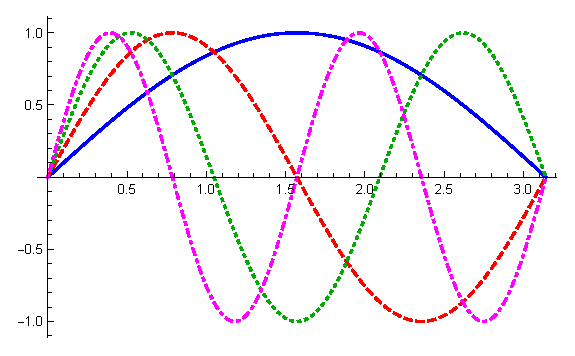
\includegraphics[scale=1]{Imagenes/Eigenfunciones_Sin_nx.eps}
\caption{Gráfica de las funciones propias $\phi_{n} (x) = \sin n \,x$ para $n = 1, 2, 3, 4$.}
\label{fig:figura_04_01}
\end{figure}
\end{frame}
\begin{frame}
\frametitle{Eigenfunciones ortogonales}
También sabemos que el conjunto $\left\{ \sin n \, x \right\}$ con $n = 1, \ldots, \infty$ es un conjunto ortogonal de funciones básicas de longitud:
\pause
\begin{align*}
\norm{\phi_{n}} = \sqrt{\dfrac{\pi}{2}}
\end{align*}
\end{frame}
\begin{frame}
\frametitle{El cociente de Rayleigh}
Por lo tanto, el cociente de Rayleigh se puede calcular usando $p(x) = 1$, $q (x) = 0$ y las funciones propias. \pause Está dado entonces por:
\pause
\begin{eqnarray}
\begin{aligned}[b]
R &= \dfrac{- \phi_{n} \, \pderivada{\phi}_{n} \eval_{0}^{\pi} + \scaleint{6ex}_{\bs 0}^{\pi} \, (\pderivada{\phi}_{n})^{2} \dd{x}}{\pi/2} = \\[0.35em] \pause
&= \dfrac{2}{\pi} \scaleint{6ex}_{\bs 0}^{\pi} \left( - n^{2} \, \cos n \, x \right)^{2} \dd{x} = \\[0.35em] \pause
&= n^{2}
\end{aligned}
\label{eq:ecuacion_04_13}
\end{eqnarray}
\end{frame}
\begin{frame}
\frametitle{El cociente de Rayleigh}
Por lo tanto, conociendo la función propia, el cociente de Rayleigh devuelve los valores propios como se esperaba.
\end{frame}
\begin{frame}
\frametitle{Ejemplo 3}
Buscamos las funciones propias del operador que se encuentran en el \textbf{Ejemplo 1}. 
\\
\bigskip
\pause
Es decir, queremos resolver el problema de los valores propios:\
\pause
\begin{align}
\mathcal{L} \, y = \left( x \, \pderivada{y} \right)^{\prime} + \dfrac{2}{x} \, y = - \lambda \, \sigma \, y
\label{eq:ecuacion_04_14}
\end{align}
sujeta a las CDF:
\begin{align*}
\pderivada{y} (1) = 0, \hspace{1cm} \pderivada{y}(2) = 0
\end{align*}
\end{frame}
\begin{frame}
\frametitle{Consideración importante}
Tomemos en cuenta que todavía no conocemos quién es la función $\sigma (x)$, pero elegiremos una función adecuada para obtener las soluciones.
\end{frame}
\begin{frame}
\frametitle{Trabajando con la derivada}
Expandiendo la derivada, tendremos que:
\pause
\begin{align*}
x \, \sderivada{y} + \pderivada{y} + \dfrac{2}{x} \, y = - \lambda \, \sigma \, y
\end{align*}
\end{frame}
\begin{frame}
\frametitle{Trabajando con la derivada}
Multiplicamos por $x$ para obtener:
\pause
\begin{align*}
x^{2} \, \sderivada{y} + x \, \pderivada{y} + (2 + \lambda \, x \,  \sigma) \, y = 0
\end{align*}
\end{frame}
\begin{frame}
\frametitle{ED familiar}
Veamos que si elegimos $\sigma(x) = x^{-1}$, entonces la ecuación se puede expresar como una ecuación de tipo Cauchy-Euler.
\\
\bigskip
\pause
Entonces tendremos:
\pause
\begin{align*}
x^{2} \, \sderivada{y} + x \, \pderivada{y} + (\lambda + 2) \, y = 0
\end{align*}
\end{frame}
\begin{frame}
\frametitle{ED familiar}
La ecuación característica es:
\pause
\begin{align*}
r^{2} + \lambda + 2 = 0
\end{align*}
\pause
Para tener soluciones oscilatorias, se necesita que $\lambda + 2 > 0$.
\end{frame}
\begin{frame}
\frametitle{Solución general}
Por lo tanto, la solución general es:
\pause
\begin{align}
y(x) = c_{1} \, \cos \left( \sqrt{\lambda + 2} \, \ln \abs{x} \right) + c_{2} \, \sin \left( \sqrt{\lambda + 2} \, \ln \abs{x} \right)
\label{eq:ecuacion_04_15}
\end{align}
\end{frame}
\begin{frame}
\frametitle{Usando las CDF}
Aplicamos las CDF $\pderivada{y}(1) = 0$, \pause obliga que $c_{2} = 0$, esto nos deja:
\pause
\begin{align*}
y(x) = c_{1} \, \cos \left( \sqrt{\lambda + 2} \, \ln \abs{x} \right)
\end{align*}
\end{frame}
\begin{frame}
\frametitle{Usando las CDF}
La segunda condición $\pderivada{y}(2) = 0$, nos lleva a:
\pause
\begin{align*}
\sin \left( \sqrt{\lambda + 2} \, \ln 2 \right) = 0
\end{align*}
\pause
Las soluciones no triviales se presentan cuando:
\pause
\begin{align*}
\sqrt{\lambda + 2} \, \ln 2 = n \, \pi \hspace{1.5cm} n = 0, 1, 2, \ldots
\end{align*}
\end{frame}
\begin{frame}
\frametitle{Eigenfunciones y eigenvalores}
Entonces se tiene que las eigenfunciones para este problema de eigen propios son:
\pause
\begin{align*}
y_{n}(x) = \cos \left( \dfrac{n \, \pi}{\ln 2} \, \ln x \right), \hspace{1.5cm} 1 \leq x \leq 2
\end{align*}
\pause
Y los valores propios son:
\pause
\begin{align*}
\lambda_{n} = \left( \dfrac{n \, \pi}{\ln 2} \right)^{2} - 2, \hspace{1.5cm} n = 0, 1, 2, \ldots
\end{align*}
\end{frame}
\begin{frame}
\frametitle{Caso importante}
\emph{Nota:} Incluimos el caso $n = 0$ porque $y (x) =$ constante, es una solución del caso $\lambda = - 2$.
\\
\bigskip
\pause
Más específicamente, en este caso la ecuación característica se reduce a $r^{2} = 0$.
\end{frame}
\begin{frame}
\frametitle{Caso importante}
Por lo tanto, la solución general de esta ecuación de Cauchy-Euler es:
\pause
\begin{align*}
y (x) = c_{1} + c_{2} \, \ln \abs{x}
\end{align*}
\end{frame}
\begin{frame}
\frametitle{Ocupando las CDF}
Haciendo que $\pderivada{y} (1) = 0$, obliga que $c_{2} = 0$.
\\
\bigskip
\pause
Por lo que $\pderivada{y} (2)$ se anula automáticamente, dejando la solución en este caso como $y(x) = c_{1}$.
\end{frame}
\begin{frame}
\frametitle{Se cumplen las propiedades}
Observamos que algunas de las propiedades enumeradas al principio de la sección son válidas para este ejemplo.
\pause
\setbeamercolor{item projected}{bg=blue!70!black,fg=yellow}
\setbeamertemplate{enumerate items}[circle]
\begin{enumerate}[<+->]
\item Los valores propios se consideran reales, contables y ordenados.
\item Hay al menos uno, $\lambda_{0} = -2$.
\item Se pueden encontrar los ceros de cada función propia en el intervalo $[1, 2]$. \pause Entonces, el argumento del coseno, $\left( \dfrac{n \, \pi}{\ln 2} \, \ln x \right)$, toma valores de $0$ a $n \pi$ para $x \in [1, 2]$. \pause La función coseno tiene $n - 1$ raíces en este intervalo.
\seti
\end{enumerate}
\end{frame}
\begin{frame}
\frametitle{Se cumplen las propiedades}
Observamos que algunas de las propiedades enumeradas al principio de la sección son válidas para este ejemplo.
\pause
\setbeamercolor{item projected}{bg=blue!70!black,fg=yellow}
\setbeamertemplate{enumerate items}[circle]
\begin{enumerate}[<+->]
\conti
\item La ortogonalidad se revisa como sigue: En la integral usamos el cambio de variable $y = \dfrac{\pi \, \ln x}{\ln 2}$.
\\
\pause
Esto nos devuelve:
\begin{eqnarray}
\begin{aligned}[b]
\langle y_{n}, y_{n} \rangle &= \scaleint{6ex}_{\bs 1}^{2} \, \cos \left( \dfrac{n \, \pi}{\ln 2} \, \ln x \right) \, \cos \left( \dfrac{m \, \pi}{\ln 2} \, \ln x \right) \dfrac{\dd{x}}{x} = \\[0.5em]
&= \dfrac{\ln 2}{\pi} \scaleint{6ex}_{\bs 0}^{\pi} \cos (n \, y) \, \cos (m \, y) \dd{y} = \\[0.5em]
&= \dfrac{\ln 2}{2} \, \delta_{nm}
\end{aligned}
\label{eq:ecuacion_04_16}
\end{eqnarray}
\end{enumerate}
\end{frame}                
\end{document}